
\paragraph{Generalised Riemann coordinates.}
We generalise to Riemann coordinates. Let $\hat u = (\hat R, \hat Q)$ be the point in $\Omega_f$ defined by $\hat Q = \hat R V$, see Figure \ref{Domain congested ph}. The point $\hat u$ lies on the continuation of the lower border of $\Omega_c$.  
For $\Omega_f$ we have \todo{$\Omega_f$ riemann coord.}\\
For $\Omega_c$ we have the right eigenvectors
\begin{align*}
    &\lambda_1 = \big ( \frac{2}{R} - \frac{1}{\rho} )\big (Q- q) - \frac{Q}{R}, \quad \quad \lambda_2 = \big(1 - \frac{\rho}{q}\big)\frac{q}{\rho} = v_c \\
    & r_1 = \begin{pmatrix} \rho \\ q - Q \end{pmatrix} \quad \quad \quad  \quad \quad \quad \quad \quad  r_2 = \begin{pmatrix} R - \rho \\ \frac{Rq}{\rho} \end{pmatrix} \\
    & \nabla \lambda_1 \cdot r_1 = 2\frac{Q-q}{R} \quad \quad \quad \quad \quad  \quad \nabla \lambda_2 \cdot r_2 = 0
\end{align*}
Note we have already found $\nabla \lambda_2 \cdot r_2 = 0$, we choose this as $\omega_1 = \lambda_2 = v_c$. For $\nabla \omega_2 \cdot r_1 = \big ( \frac{\partial \omega_2}{\partial \rho}, \frac{\partial \omega_2}{\partial q} \big ) \cdot \begin{pmatrix} \rho \\ q - Q \end{pmatrix} = 0 $ we see that by choosing  $\frac{\partial \omega_2}{\partial \rho} = - \frac{ q-Q }{\rho}$ and $ \frac{\partial \omega_2}{\partial q} =  \frac{1}{\rho} $ the expressions cancel. Now we have    $\omega_2 = \frac{q-Q}{\rho}$, which is a desirable result as it the slope of the first family wave. 

Now we have the Riemann coordinates
\begin{align*}
    \omega_1 = \begin{cases}
    v_c(\rho, q), (\rho, q) \in \Omega_c \\
    V_f, (\rho, q) \in \Omega_f
    \end{cases}
    \omega_2 = \begin{cases}
    \frac{q-Q}{\rho}, (\rho, q) \in \Omega_c \\
    \frac{q-Q}{\rho}, (\rho, q) \in \Omega_f, \rho \geq \hat R \\
    v_f(\rho) - v_f(\hat R) + \frac{\hat Q - Q}{\hat R }, (\rho, q) \in \Omega_f, \rho \leq \hat R \\
    \end{cases}
\end{align*}

%We continue by finding the direction of the rarefaction and shock in the new coordinate system. 
\begin{figure}[H] \centering 
\begin{minipage}{.35\textwidth}
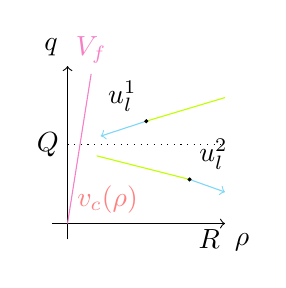
\begin{tikzpicture}
% coordinates
\draw[->] (0,-0.2) -- (0,2) node[anchor= south east] {$q$};
\draw[->] (-0.2,0) -- (2,0) node[anchor= north west] {$\rho$};
% rarefactions
\draw[<-][cyan!50] (0.42, 1.11) -- (1, 1.3) ;
\draw[lime] (1, 1.3) -- (2, 1.6) ;

\draw[->][cyan!50] (1.55,0.56)  -- (2, 0.4) ;
\draw[-][lime] (0.37, 0.86) -- (1.55,0.56)  ;


% v_c
\draw[red!50, domain=0:0.69]  plot[id=x] function{x*(3*x+1)}  node[anchor= south west] {$v_c(\rho)$};
% V_f
\draw[magenta!50] (0,0) -- (0.3, 1.9);
\node[magenta!50] at (0.3, 2.2) {$V_f$};

\draw[dotted] (0,1) -- (2, 1);

\filldraw[black] (1,1.3) circle (0.5pt) node[anchor = south east]{$u_l^1$} ;
\filldraw[black] (1.55,0.56) circle (0.5pt) node[anchor = south west]{$u_l^2$} ;
% contacts
\draw[ orange!50, domain=0:1.86]  plot[id=x] function{(x/1.38)*(2-1.38)/(2-x)*0.33};
\draw[ orange!50, domain=0:1.28]  plot[id=x] function{(x/1.16)*(2-1.16)/(2-x)*1.63};
%
%\node at (1, 1.55) {$u_l$};
\node at (1.8, -0.2) {$R$};
\node at (-0.25, 1) {$Q$};
\end{tikzpicture}
\caption{Wave solutions from two starting points $u_l^1$ and $u_l^2$. }
\label{Fig:FullSol_ic_rhoq}
\end{minipage}
\quad \quad \quad \quad 
\begin{minipage}{.35\textwidth}
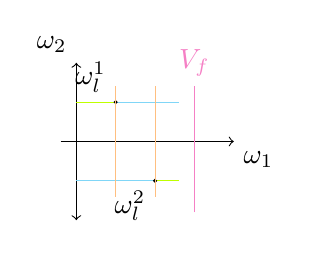
\begin{tikzpicture}
% coordinates
\draw[<->] (0,0) -- (0,2) node[anchor= south east] {$\omega_2$};
\draw[->] (-0.2,1) -- (2,1) node[anchor= north west] {$\omega_1$};
% rarefactions
% rarefactions
\draw[lime] (0, 1.5) -- (0.5, 1.5) ;
\draw[cyan!50] (0.5, 1.5) -- (1.3, 1.5)  ;
\filldraw[black] (0.5, 1.5) circle (0.5pt) node[anchor = south east]{$\omega_l^1$} ;

\draw[cyan!50] (0, 0.5) -- (1, 0.5) ;
\draw[lime] (1, 0.5) -- (1.3, 0.5) ;
\filldraw[black] (1, 0.5)  circle (0.5pt) node[anchor = north east]{$\omega_l^2$} ;

% contacts
\draw[orange!50] (0.5, 1.7) -- (0.5, 0.3) ;
\draw[orange!50] (1, 1.7) -- (1, 0.3) ;

% free ph line
\draw[magenta!50] (1.5, 0.1) -- (1.5, 1.7); 
\node[magenta!50] at (1.5, 2) {$V_f$};
%\filldraw[black] (1.5, 1.5)  circle (0.5pt) node[anchor =  west]{$\omega_r^2$} ;
%\filldraw[black] (1.5, 0.5)  circle (0.5pt) node[anchor = west]{$\omega_r^2$} ;

\end{tikzpicture}
\caption{Wave solutions from two starting points $\omega_l^1$ and $\omega_l^2$.}
\label{Fig:FullSol_ic_ww}
\end{minipage}
\end{figure}

% -----------------------------------------------------------
% -----------------------------------------------------------
% -----------------------------------------------------------
\begin{comment}

From Figure \ref{Fig:FullSol_ic_rhoq}, observe that
\begin{align*}
    q > Q \begin{cases}
    q \searrow rarefaction\\
    q \nearrow shock
    \end{cases}
    q < Q \begin{cases}
    q \searrow shock \\
    q \nearrow rarefaction
    \end{cases}
\end{align*}

Using the relation between the coordinates $\rho, q$ and $\omega_1, \omega_2$ 
\begin{itemize}
    \item $\omega_2 > 0$ 
    $\rho$ const. $q \searrow \leftrightarrow \omega_1, \omega_2 \searrow$ rarefaction
    \item $\omega_2 < 0$ 
    $\rho$ const. $q \searrow \leftrightarrow \omega_1, \omega_2 \searrow$ shock
\end{itemize}

Which means we have the relation between shock and rarefaction in $\omega$-coordinates, the result can be seen in Figure \ref{Fig:FullSol_ic_ww}
\begin{align*}
    \omega_2 > 0 \begin{cases}
    \omega_2 \searrow rarefaction\\
    \omega_2 \nearrow shock
    \end{cases}
    \omega_2 < 0\begin{cases}
    \omega_2 \searrow shock \\
    \omega_2 \nearrow rarefaction
    \end{cases}
\end{align*}
\end{comment}